\section{Hertzscher Dipol}

Als erstes Thema werden Dipolantennen beschrieben. Dabei wird vor allem auf den Hertzschen Dipol eingegangen, welcher das Modell der Antenne durch seine kurze Länge vereinfacht.

\subsection{Theorie}\label{sec:HerDip}

Eine Dipol Antenne kann als kurzer Linearstrahler beschrieben werden, wobei dessen länge $l \ll \lambda_0 /4$ beträgt. $\lambda_0$ beschreibt dabei die Wellenlänge, welche durch das Verhältnis der Lichtgeschwindigkeit zur Signalfrequenz $c_0/f$ beschreibt. 

xxx

Ein solcher Strahler ist in Abbildung xxx zu sehen, wobei $\underline{I}$ der komplexe Strom einer Sinusschwingung darstellt, welche konstant über die gesamte Länge schwingt. $\phi$ stellt den Winkel dar, welcher um die z-Achse rotiert und über die x- und y-Achse aufgespannt ist.$\theta$ hingegen rotiert um die x-Achse und wird über die y- und z-Achse aufgespannt. Für die Kugelkoordinaten bedeutet dies, dass mit den Restriktionen 

\begin{align}
&0 \leq \varphi \leq 2\pi\\
&0 \leq \vartheta \leq \pi \label{eq:HertzTheta}
\end{align}

der gesamte Bereich des Koordinatensystems abgedeckt ist. Das durch den Strom induzierte Magnetfeld kann mit 

\begin{equation}
\underline{H}_0 = j\pi \frac{\underline{I}l}{{\lambda_0}^2}
\end{equation}

beschrieben werden, was für zwei Formeln für das magnetische und elektrische Feld liefert:

\begin{align}
\underline{H}_\varphi   &= \underline{H}_0 \sin \vartheta \frac{e^{-jk_0r}}{k_0r}\\
\underline{E}_\vartheta &= Z_0 \underline{H}_\varphi = Z_0 \underline{H}_0 \sin \vartheta \frac{e^{-jk_0r}}{k_0r}.\label{eq:HertzE}
\end{align}

Hierbei beschreibt $r$ die Distanz des Punktes zu Ursprung und $k_0 = \omega \sqrt{\mu_0 \eta_0} = c_0/\omega$ die Wellenzahl im Vakuum beschreibt. Somit beschreibt die komplexe Exponentialfunktion die Ausbreitung der Welle, was mit der Theorie der Wellenleitern übereinstimmt. Im Nenner ist das Abklingen des Sinus zu erkennen, welches abhängig von der Distanz zum Ursprung und der Wellenzahl ist. xxx

\subsection{Richtdiagramm}

Ein wichtiges Diagramm für die Analyse von Antennen ist das Richtdiagramm. Mit diesem kann die Direktivität einer Antenne dargestellt werden, welche mitteilt, in welche Richtung wie viel der Leistung der Antenne abgestrahlt wird. Diese Analyse geschieht im Fernfeld, was bedeutet dass die Annahme $r \rightarrow \infty$ getroffen wird. Somit kann verhindert werden, dass eine Antenne in eine unerwünschte Richtung Leistung abgibt und somit eine andere Antenne stören könnte. Daher wird die Feldstärke einer Antenne in Abhängigkeit der Raumrichtung beschreiben, welche mit den Kugelkoordinaten $\varphi$ und $\vartheta$ angegeben wird.\\

Für das Richtdiagramm wird die komplexe elektrische Feldstärke in den Kugelkoordinaten auf dessen maximale Feldstärke normiert, wobei sich dadurch ein wert zwischen $0$ und $1$ einstellt. Dies ergibt die auf den Maximalwert normierte Winkelverteilung des elektrischen Feldes. Diese Kenngrösse wird als Richtcharakteristik bezeichnet:

\begin{equation}
C(\vartheta,\varphi) = \frac{|\underline{E}(\vartheta,\varphi)|}{|\underline{E}(\vartheta,\varphi)|_{\mathrm{max}}}.
\end{equation}

Als Beispiel wird der Hertzsche Dipol aus dem Abschnitt \ref{sec:HerDip} betrachtet. Dessen elektrische Feldstärke ist in Formel \ref{eq:HertzE} beschrieben, wobei durch den Sinus dessen Maximalwert direkt bestimmt werden kann. Somit ergibt sich für die Richtcharakteristik:

\begin{equation}\label{eq:HertRicht}
C(\vartheta,\varphi) = \frac{|\underline{E}(\vartheta,\varphi)|}{|\underline{E}(\vartheta,\varphi)|_{\mathrm{max}}} = \frac{\frac{Z_0 |\underline{H}_0| |\sin \vartheta|}{k_0r}}{\frac{Z_0 |\underline{H}_0|}{k_0r}} = \sin \vartheta.
\end{equation}

Aus Formel \ref{eq:HertRicht} ist herauszulesen, dass an der Stellen für $\vartheta$ gleich Null oder $\pi$ eine Nullstelle ist, das Maximum an der Stelle $\pi/2$ mit dem normierten Wert 1 erreicht wird und bei $\pi/4$ der Wert $1/\sqrt{2}$ anliegt.\\

Zur Verifikation wurde zuerst ein MATLAB-Code erstellt, welcher die Polarkoordinaten darstellen soll.

\begin{lstlisting}
%Richtcharakteristik.m

%Thomas Frei & Simon Zoller

%Kugelkoordinaten
theta=0:0.01:2*pi;
phi = 0:0.01:2*pi;

%Richtcharakteristik
C = cell(6);

%Titel
plotTitle = cell(6);
plotTitle{1} = 'Vertikales Richtdiagramm z-Dipol';
plotTitle{2} = 'Horizontales Richtdiagramm z-Dipol';
plotTitle{3} = 'Vertikales Richtdiagramm x-Dipol';
plotTitle{4} = 'Horizontales Richtdiagramm x-Dipol';
plotTitle{5} = 'Vertikales Richtdiagramm y-Dipol';
plotTitle{6} = 'Horizontales Richtdiagramm y-Dipol';

%z-Dipol
C{1} = abs(sin(theta));
C{2} = ones(size(theta));

%x-Dipol
C{3} = abs(sqrt(1-sin(theta).^2.*cos(pi/2).^2));
C{4} = abs(sqrt(1-sin(pi/2).^2.*cos(phi).^2));

%y-Dipol
C{5} = abs(sqrt(1-sin(theta).^2.*sin(pi).^2));
C{6} = abs(sqrt(1-sin(pi/2).^2.*sin(phi).^2));

%Plot in Schleife
for ind=1:6
    subplot(3, 2, ind) ;
    polarplot(theta,C{ind});
    pax = gca;
    pax.ThetaDir = 'clockwise';
    pax.ThetaZeroLocation = 'top';
    rlim([0 1]);
    title(plotTitle{ind});
end
\end{lstlisting}

\begin{figure}[!ht]
	\centering
    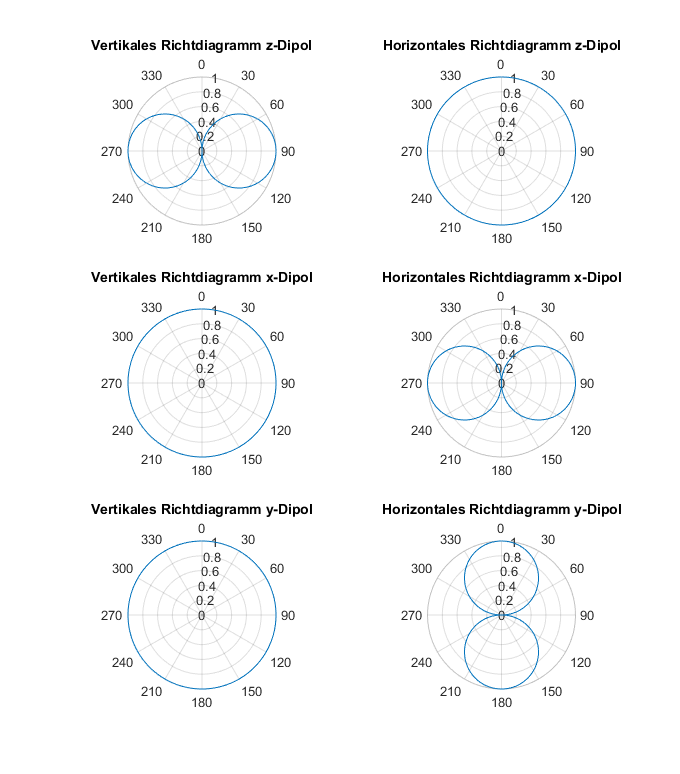
\includegraphics[width=\textwidth]{HertzscherDipol.png}
    \caption{Simulationen des Hertzschen Dipoles mit der Anordnung in allen drei verschiedenen Achsenrichtungen.}
    \label{fig:HertzscherDipol}
\end{figure}

Das Resultat ist in Figur \ref{fig:HertzscherDipol} zu sehen. Die Werte stimmen mit den Annahmen überein und auch mit der erwarteten Figur xxx. Zu beachten ist jedoch, dass nur ein Kreis ersichtlich ist, da wie in Formel \ref{eq:HertzTheta} definiert $\vartheta$ nur über den halben Bereich gilt. Das Resultat in Figur xxx ist dreidimensional angegeben. Meistens reicht es jedoch, einen Schnitt der Charakteristik anzugeben. Dabei wird unter dem vertikalen und horizontalen Richtdiagramm unterschieden, wobei für das vertikale Diagramm mit $C(\vartheta, \varphi = \varphi_0)$ die Strahlung im Elevationswinkel $\vartheta$ angegeben wird (wie in Figur xxx) und beim horizontalen Diagramm mit $C(\vartheta=\pi/2, \varphi)$ die Strahlung im sogenannten Azimutwinkel $\varphi$ angegeben wird. Dies resultiert in der E-Ebene für das vertikale Diagramm und in der H-Ebene für das horizontale Diagramm des z-Dipols.\\

Als letzter Teil der Theorie wird auf die Halbwertsbreiten $\Delta \vartheta$ und $\Delta \varphi$ eingegangen. Diese beschreiben die Breite der Hauptkeule, wobei der Winkel unter welchem die Hälfte der Strahlungsdichte liegt angegeben wird (beziehungsweise der -3dB Punkt). Da wie schon erwähnt beim Hertschen Dipol bei $\pi/4$ die Richtcharakteristik $1/\sqrt{2}$ beträgt, ergibt sich für die Halbwertsbreiten einen Winkel von \SI{90}{\degree}.

\subsection{Simulation}

